\documentclass[tikz,border=10pt]{standalone}
\usepackage{url}

\usetikzlibrary{arrows.meta, positioning, shapes.geometric, shapes.misc, fit, backgrounds, calc, matrix}

\tikzset{
    >=Latex,
    font=\sffamily\large,
    node distance=1.5cm and 3cm,
    dag_result/.style={
        rectangle,
        draw=green!70!black,
        fill=green!15,
        very thick,
        minimum width=4.5cm,
        minimum height=1.5cm,
        text width=5cm,
        align=center
    },
    dag_lemma/.style={
        rounded rectangle,
        draw=orange!80!black,
        fill=yellow!20,
        very thick,
        minimum width=4.5cm,
        minimum height=1.5cm,
        text width=5cm,
        align=center
    },
    dag_model/.style={
        ellipse,
        draw=blue!70!black,
        fill=blue!12,
        very thick,
        minimum width=4.5cm,
        minimum height=1.5cm,
        text width=4.5cm,
        align=center
    },
    dag_unformalized/.style={
        rectangle,
        draw=gray!60!black,
        fill=gray!10,
        very thick,
        dashed,
        minimum width=4.5cm,
        minimum height=1.5cm,
        text width=5cm,
        align=center
    },
    dag_conditional/.style={
        rectangle,
        rounded corners,
        draw=orange!80!black,
        fill=orange!10,
        very thick,
        minimum width=4.5cm,
        minimum height=1.5cm,
        text width=5cm,
        align=center
    },
    dag_partial/.style={
        rectangle,
        rounded corners,
        draw=yellow!55!black,
        fill=yellow!10,
        very thick,
        dashed,
        minimum width=4.5cm,
        minimum height=1.5cm,
        text width=5cm,
        align=center
    },
    dag_scaffold/.style={
        rectangle,
        draw=gray!55!black,
        fill=white,
        very thick,
        dotted,
        minimum width=4.5cm,
        minimum height=1.5cm,
        text width=5cm,
        align=center
    },
    dag_caveat/.style={
        diamond,
        draw=red!70!black,
        fill=red!10,
        minimum width=4cm,
        align=center,
        inner sep=0pt,
        font=\sffamily\small
    },
    % Lean-checked formal dependency edge. Use only for dependencies that are
    % discharged in the Lean proof path represented by the target node.
    dag_arrow/.style={
        -{Latex[length=3.0mm,width=2.1mm]},
        very thick,
        shorten >=1.5pt,
        shorten <=1.5pt
    },
    % Non-closed or non-required roadmap edge: unresolved, conditional, caveat,
    % paper-route, or explicitly bypassed dependency.
    dag_dashed_arrow/.style={
        -{Latex[length=3.0mm,width=2.1mm]},
        very thick,
        dashed,
        shorten >=1.5pt,
        shorten <=1.5pt
    },
    dag_template_legend/.style={
        outer sep=0pt,
        minimum width=3cm,
        minimum height=1.25cm,
        text width=2.72cm,
        inner sep=2pt,
        font=\sffamily\scriptsize,
        align=center
    },
    dag_caveat_legend/.style={
        dag_caveat,
        dag_template_legend,
        minimum width=2.15cm,
        minimum height=0.9cm,
        text width=1.9cm,
        inner sep=1pt,
        font=\sffamily\tiny
    },
    dag_template_note/.style={
        rectangle,
        draw=gray!50,
        fill=gray!5,
        rounded corners,
        text width=13cm,
        align=left,
        font=\sffamily\small,
        inner sep=6pt
    }
}

% Legend Helper
\newcommand{\daglegend}[2]{
  \node[
    draw,
    rounded corners,
    very thick,
    fill=none,
    fit=#1,
    inner sep=10pt,
    outer sep=0pt,
    % keep label handling explicit below
  ] (#2) {};
  \coordinate (dagLegendSouthWest) at (#2.south west);
  \node[
    font=\sffamily\bfseries\large,
    fill=white,
    anchor=south west,
    inner sep=1pt
  ] at ($(#2.north west) + (0.08cm,0.06cm)$) {Legend};
}

\newcommand{\daglegendAtTopLeft}[2]{
    \node[draw, rounded corners, very thick, fit=#1, inner sep=12pt, label=above:\textbf{\Large Legend}] (#2) {};
}

\newcommand{\dagPaperMetadata}[5]{
  \node[
    align=left,
    font=\sffamily\small,
    text width=15cm,
    minimum width=15cm,
    inner sep=0pt,
    outer sep=0pt,
    anchor=north west,
    name=dagPaperMetadata
  ] at (0,0) {
    \textbf{Paper:} #1\\
    \textbf{Authors:} #2\\
    \textbf{Publication venue:} #3\\
    \textbf{Year:} #4\\
    \if\relax\detokenize{#5}\relax\relax\else
      \textbf{Formalized PDF:} \url{#5}
    \fi
  };
}

\newcommand{\dagPaperLegendRightOfMetadata}[1]{
  \begin{scope}[shift={($(dagPaperMetadata.north east) + (2.20cm,-2.10cm)$)}]
    #1
  \end{scope}
}

\newenvironment{dagPaperBody}{
  \coordinate (dagPaperGraphStart) at ($(dagPaperMetadata.south west |- dagLegendSouthWest) + (2.60cm,-1.35cm)$);
  \begin{scope}[shift={(dagPaperGraphStart)}]
}{
  \end{scope}
}

\begin{document}
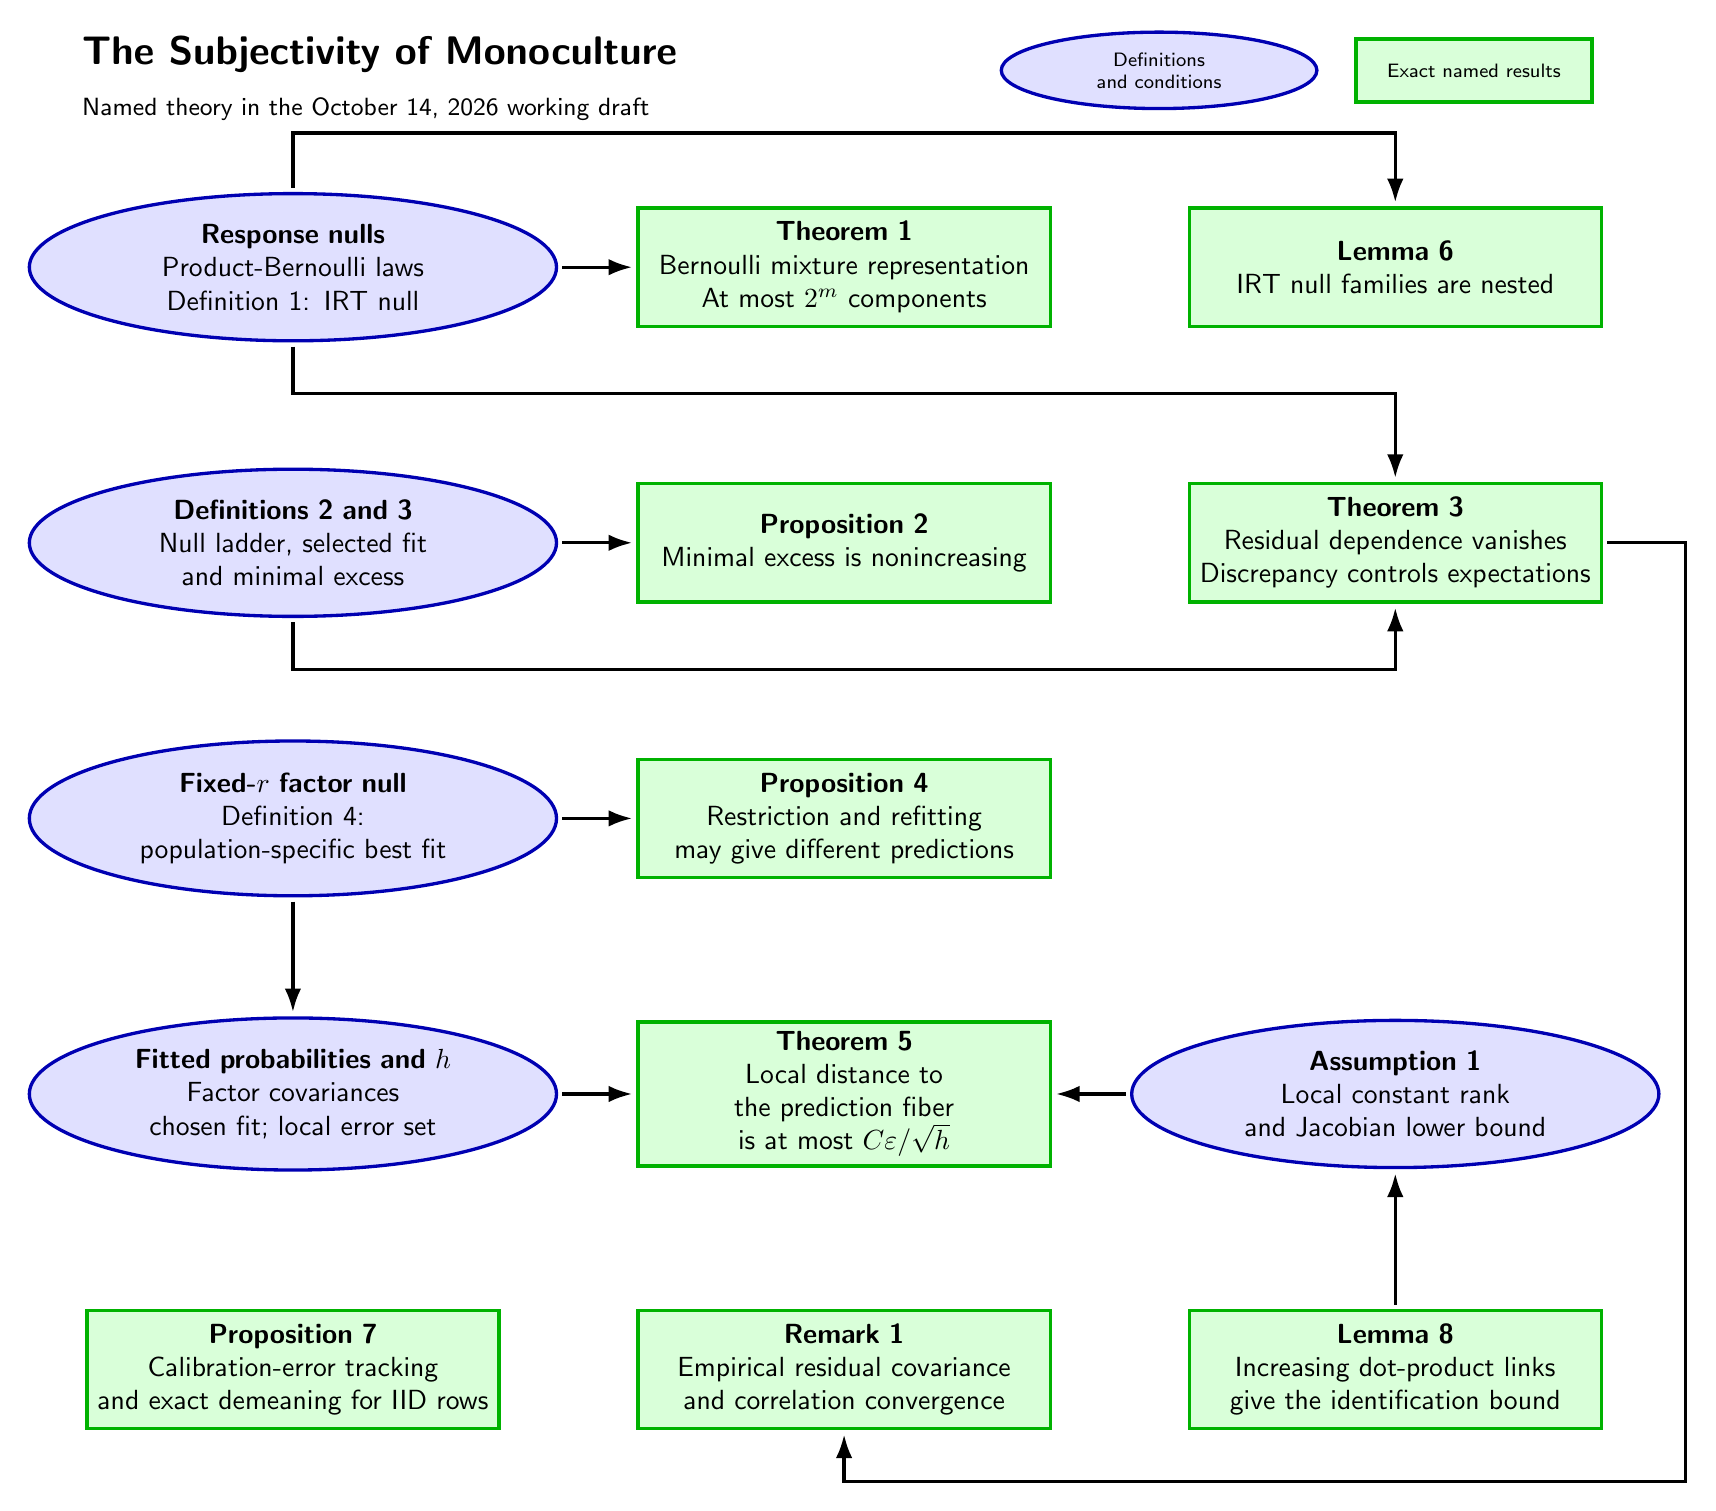
\begin{tikzpicture}[x=1cm,y=1cm,font=\sffamily\normalsize]
\node[anchor=west,font=\sffamily\bfseries\Large] at (-2.8,2.7)
  {The Subjectivity of Monoculture};
\node[anchor=west,font=\sffamily\small] at (-2.8,2.0)
  {Named theory in the October 14, 2026 working draft};
\node[dag_model,text width=2.6cm,minimum width=3cm,minimum height=0.8cm,
      font=\sffamily\scriptsize] at (11.0,2.5) {Definitions and conditions};
\node[dag_result,text width=2.6cm,minimum width=3cm,minimum height=0.8cm,
      font=\sffamily\scriptsize] at (15.0,2.5) {Exact named results};

\node[dag_model] (Null) at (0,0)
  {\textbf{Response nulls}\\Product-Bernoulli laws\\Definition 1: IRT null};
\node[dag_result] (Mixture) at (7,0)
  {\textbf{Theorem 1}\\Bernoulli mixture representation\\At most $2^m$ components};
\node[dag_result] (Nested) at (14,0)
  {\textbf{Lemma 6}\\IRT null families are nested};

\node[dag_model] (Ladder) at (0,-3.5)
  {\textbf{Definitions 2 and 3}\\Null ladder, selected fit\\and minimal excess};
\node[dag_result] (Absorption) at (7,-3.5)
  {\textbf{Proposition 2}\\Minimal excess is nonincreasing};
\node[dag_result] (Residual) at (14,-3.5)
  {\textbf{Theorem 3}\\Residual dependence vanishes\\Discrepancy controls expectations};

\node[dag_model] (Population) at (0,-7)
  {\textbf{Fixed-$r$ factor null}\\Definition 4:\\population-specific best fit};
\node[dag_result] (Relativity) at (7,-7)
  {\textbf{Proposition 4}\\Restriction and refitting\\may give different predictions};

\node[dag_model] (Heterogeneity) at (0,-10.5)
  {\textbf{Fitted probabilities and $h$}\\Factor covariances\\chosen fit; local error set};
\node[dag_result] (Stability) at (7,-10.5)
  {\textbf{Theorem 5}\\Local distance to the prediction fiber\\is at most $C\varepsilon/\sqrt h$};
\node[dag_model] (Identification) at (14,-10.5)
  {\textbf{Assumption 1}\\Local constant rank\\and Jacobian lower bound};

\node[dag_result] (Debiasing) at (0,-14)
  {\textbf{Proposition 7}\\Calibration-error tracking\\and exact demeaning for IID rows};
\node[dag_result] (Empirical) at (7,-14)
  {\textbf{Remark 1}\\Empirical residual covariance\\and correlation convergence};
\node[dag_result] (IRTIdentification) at (14,-14)
  {\textbf{Lemma 8}\\Increasing dot-product links\\give the identification bound};

\draw[dag_arrow] (Null) -- (Mixture);
\draw[dag_arrow] (Null.north) -- ++(0,0.75) -| (Nested.north);
\draw[dag_arrow] (Ladder) -- (Absorption);
\draw[dag_arrow] (Null.south) -- ++(0,-0.65) -| (Residual.north);
\draw[dag_arrow] (Ladder.south) -- ++(0,-0.65) -| (Residual.south);
\draw[dag_arrow] (Population) -- (Relativity);
\draw[dag_arrow] (Population) -- (Heterogeneity);
\draw[dag_arrow] (Heterogeneity) -- (Stability);
\draw[dag_arrow] (Identification) -- (Stability);
\draw[dag_arrow] (IRTIdentification) -- (Identification);
\draw[dag_arrow] (Residual.east) -- ++(1.05,0)
  |- ($(Empirical.south)+(0,-0.65)$) -- (Empirical.south);
\end{tikzpicture}
\end{document}
